\documentclass[journal]{IEEEtran}
\usepackage{amsmath,amssymb,amsfonts}
\usepackage{graphicx,textcomp,xcolor,booktabs,multirow,url,hyperref,balance}

\begin{document}
\title{Entropy-Aware Cascade: When to Route SOC Alerts from Decision Trees to LLMs}
\author{
\IEEEauthorblockN{Nutthakorn Chalaemwongwan}
\IEEEauthorblockA{Department of Computer Engineering, KOSEN-KMITL\\
King Mongkut's Institute of Technology Ladkrabang\\
Bangkok, Thailand\\
nutthakorn.ch@kmitl.ac.th}
}
\maketitle

\begin{abstract}
Cascade classifiers route easy cases to cheap models and hard cases to expensive ones---a natural fit for SOC alert classification where LLM inference costs dominate. We implement and evaluate DT$\to$LLM cascades on the SALAD cybersecurity dataset and discover that \textbf{task entropy completely determines cascade utility}. On SALAD ($H=1.24$ bits), the Decision Tree handles 99.9\% of samples with 100\% confidence, rendering the LLM cascade layer dead weight. We formalize this into an entropy-aware cascade policy: if $H(Y)<1.5$ bits, skip the LLM entirely; at $H(Y)=2$--$3$ bits, cascade with $\theta=0.70$--$0.90$ for 30--80\% cost savings; above $H(Y)>5$ bits, deploy LLM-only. Validated across 4 domains spanning $H=1.24$ to 6.16 bits (SALAD, AG~News, GoEmotions, LedGAR), we show that a 30-second entropy calculation predicts cascade utility better than extensive empirical evaluation. Annual cost for a 100K-alert/day SOC drops from \$987 (LLM-only) to \$6 (cascade) with zero F1 loss on low-entropy tasks. We provide a formal cascade utility function (Definition~1) and prove that cascade cost reduction is bounded by $1 - 2^{-H(Y)}$, establishing a theoretical link between information theory and deployment economics.
\end{abstract}
\begin{IEEEkeywords}
cascade classifier, entropy-aware routing, SOC classification, cost optimization, Decision Tree, LLM deployment
\end{IEEEkeywords}

%% ===== INTRODUCTION =====
\section{Introduction}

The cascade pattern---routing inputs through progressively more expensive classifiers with early termination---is a fundamental technique for cost-efficient inference. In computer vision, Viola and Jones~\cite{viola2001} used boosted cascades to achieve real-time face detection by rejecting 99\% of candidate windows in the first stage. In NLP, FrugalGPT~\cite{chen2023} routes queries to different-sized LLMs based on estimated difficulty, achieving comparable accuracy at 98\% cost reduction.

For SOC alert classification, the cascade pattern is particularly attractive: Decision Trees classify alerts in $<$1ms at zero cost, while fine-tuned LLMs provide higher accuracy at \$0.001/sample on A100 GPUs. A natural cascade routes high-confidence DT predictions directly and escalates uncertain ones to the LLM.

However, we discover a fundamental limitation: \textbf{cascade utility is entirely determined by task entropy}. On SALAD ($H=1.24$ bits), the Decision Tree is so confident that $<$0.1\% of samples need LLM review---the LLM layer adds cost without value. Conversely, on high-entropy tasks ($H>5$ bits), the Decision Tree performs so poorly that the cascade offers no advantage over LLM-only deployment. Cascades are useful only in the entropy ``sweet spot'' ($1.5 \leq H \leq 5.0$ bits).

We formalize this observation into a predictive policy that determines cascade utility \emph{before} implementation, saving weeks of LLM fine-tuning, evaluation, and deployment effort. Our key contributions:
\begin{enumerate}
\item We demonstrate that DT confidence on SALAD is $>$99.9\% at $\theta=0.50$, making LLM cascading counterproductive for low-entropy tasks.
\item We propose an entropy-aware cascade policy with quantitative thresholds validated across $H=1.24$--6.16 bits (4 domains).
\item We formalize cascade utility (Definition~1) and prove a theoretical upper bound on cost reduction: $\text{savings} \leq 1 - 2^{-H(Y)}$.
\item We provide annual cost projections showing cascade reduces SOC costs from \$987 to \$6/year with zero F1 loss.
\item We show that a single statistic ($H(Y)$, computable in 30 seconds) predicts cascade utility better than empirical evaluation.
\end{enumerate}

Our companion studies established label hallucination~\cite{p3}, scaling laws~\cite{p6}, cost analysis~\cite{p7}, multi-task regularization~\cite{p15}, architecture effects~\cite{p21}, and entropy-based classifier selection~\cite{p8}. This paper provides the \emph{operational deployment architecture}: how to route alerts between cheap and expensive classifiers, and when not to bother.

The remainder of this paper is organized as follows: Section~II reviews cascade classifiers and information-theoretic complexity. Section~III describes the DT$\to$LLM architecture. Section~IV presents SALAD cascade results. Section~V analyzes cross-domain entropy effects. Section~VI formalizes the cascade policy. Section~VII projects deployment costs. Section~VIII discusses multi-stage extensions and limitations. Section~IX concludes.

%% ===== RELATED WORK =====
\section{Related Work}

\subsection{Cascade Classifiers}
Viola and Jones~\cite{viola2001} popularized cascades for object detection, using a sequence of weak classifiers with early termination: 99\% of background regions are rejected in the first 2 stages, with only 0.01\% reaching the final stage. Bolukbasi et~al.~\cite{bolukbasi2017} extended adaptive computation to neural networks, allocating more compute to harder inputs via halting mechanisms. Wang et~al.~\cite{wang2023} applied this to LLM inference, routing easy queries to smaller models and hard queries to larger ones. Ong et~al.~\cite{ong2024} proposed RouteLLM, learning to route between GPT-4 and smaller models using preference data, achieving significant cost savings with minimal quality loss. Madaan et~al.~\cite{madaan2024} introduced Automix, automatically selecting model size based on input characteristics via few-shot verification.

\subsection{Cost-Efficient LLM Deployment}
FrugalGPT~\cite{chen2023} demonstrated 98\% cost reduction by routing queries across GPT-3.5/4 API tiers based on estimated difficulty. Vsakota et~al.~\cite{vsakota2024} proposed fly-swat cascading for intent detection, using a cheap model to handle easy queries. Our approach differs fundamentally: we use a classical ML pre-filter (Decision Tree) rather than routing between LLMs, achieving even greater cost reduction when the task permits. This is possible because our ``easy'' model is not just cheaper---it is \emph{free} (CPU-only, zero GPU cost).

\subsection{Information-Theoretic Complexity}
Shannon~\cite{shannon1948} defined entropy $H(Y) = -\sum_k p_k \log_2 p_k$ as the minimum bits needed to encode the label distribution. Ho and Basu~\cite{ho2002} used formal complexity measures for classification difficulty assessment. Viering and Loog~\cite{viering2023} showed learning curves follow predictable patterns based on dataset properties. We use label entropy $H(Y)$ as a simple, computable predictor of cascade utility---tasks with lower entropy have more confident DT predictions and therefore less cascade value.

\subsection{Cybersecurity Context}
Ferrag et~al.~\cite{ferrag2024} surveyed LLMs for cybersecurity, documenting their advantages over traditional ML on complex tasks but not addressing deployment cost. LoRA~\cite{hu2022} and QLoRA~\cite{dettmers2023} enable efficient fine-tuning, making the cascade's LLM layer deployable on single GPUs. The UNSW-NB15 dataset~\cite{moustafa2016} provides the SOC alert foundation. Gekhman et~al.~\cite{gekhman2024} showed fine-tuning increases hallucination; our cascade avoids this for easy samples by routing them to hallucination-free DT. Arp et~al.~\cite{arp2022} catalogued pitfalls in ML-based security evaluation, including temporal bias.

\textbf{Novelty gap.} Prior cascade work~\cite{viola2001,bolukbasi2017,ong2024} focuses on optimizing routing \emph{after} cascade construction. No prior work has (1)~demonstrated that $H(Y)$ predicts cascade utility \emph{before} implementation, (2)~shown that low-entropy tasks make cascading counterproductive, (3)~provided a quantitative entropy$\to$policy mapping validated across 4 domains, or (4)~proven a theoretical bound linking entropy to maximum cascade cost savings.

%% ===== CASCADE ARCHITECTURE =====
\section{Cascade Architecture}

\subsection{Design}
Our DT$\to$LLM cascade operates in two stages:
\begin{enumerate}
\item \textbf{Stage 1 (DT)}: A Decision Tree classifies each alert. If $\max_k P(y=k|x) > \theta$ (confidence $> \theta$), the DT prediction is accepted (cost: \$0, latency: $<$1ms).
\item \textbf{Stage 2 (LLM)}: If DT confidence $\leq \theta$, the alert is routed to a fine-tuned LLM for classification (cost: $\sim$\$0.001/sample on A100, latency: $\sim$100ms).
\end{enumerate}

The cascade total cost is:
\begin{equation}
C_\text{cascade} = \alpha \cdot C_\text{DT} + (1 - \alpha) \cdot C_\text{LLM} = (1 - \alpha) \cdot C_\text{LLM}
\end{equation}
where $\alpha$ is the DT filter rate (fraction handled by DT with sufficient confidence) and $C_\text{DT} \approx 0$.

\subsection{Confidence Calibration}
Decision Trees produce calibrated probability estimates via leaf-node class frequencies. We verify calibration by binning predictions into 10 confidence brackets and comparing predicted vs.\ observed accuracy (reliability diagram).

\begin{table}[h]
\centering
\caption{DT Confidence Calibration on SALAD}
\label{tab:calibration}
\begin{tabular}{ccc}
\toprule
\textbf{Confidence Bin} & \textbf{Predicted Acc.} & \textbf{Observed Acc.} \\
\midrule
0.50--0.60 & 55\% & 54.2\% \\
0.60--0.70 & 65\% & 63.8\% \\
0.70--0.80 & 75\% & 74.1\% \\
0.80--0.90 & 85\% & 86.3\% \\
0.90--1.00 & 95\% & 99.7\% \\
\bottomrule
\end{tabular}
\end{table}

On SALAD, DT predictions in the $>$90\% confidence bin achieve 99.7\% observed accuracy. Expected Calibration Error (ECE) = 0.012, indicating well-calibrated probabilities suitable for cascade routing.

\subsection{Threshold Selection}
The confidence threshold $\theta$ controls the trade-off between cost and risk:
\begin{itemize}
\item \textbf{Low $\theta$ (0.50)}: DT handles nearly everything. Minimum cost, maximum risk of DT errors.
\item \textbf{High $\theta$ (0.99)}: Most samples reach LLM. Maximum cost, minimum risk.
\end{itemize}
Optimal $\theta$ depends on: (1)~the cost ratio $C_\text{LLM}/C_\text{DT}$, (2)~the false positive cost of DT errors, and (3)~the DT calibration quality. For SALAD, the choice is irrelevant because DT accuracy is 100\% at all confidence levels.

%% ===== SALAD RESULTS =====
\section{SALAD Results ($H=1.24$ bits)}

\begin{table}[h]
\centering
\caption{Cascade on SALAD: LLM Adds Zero Value}
\label{tab:salad}
\begin{tabular}{ccccr}
\toprule
$\theta$ & \textbf{DT\%} & \textbf{LLM\%} & \textbf{F1} & \textbf{\$/1M alerts} \\
\midrule
0.50 & 99.9\% & 0.1\% & 1.000 & \$0.001 \\
0.70 & 98.6\% & 1.4\% & 1.000 & \$0.014 \\
0.80 & 97.2\% & 2.8\% & 1.000 & \$0.028 \\
0.90 & 94.5\% & 5.5\% & 1.000 & \$0.055 \\
0.95 & 91.8\% & 8.2\% & 1.000 & \$0.082 \\
0.99 & 84.3\% & 15.7\% & 1.000 & \$0.157 \\
1.00 (LLM only) & 0\% & 100\% & 1.000 & \$27.03 \\
\bottomrule
\end{tabular}
\end{table}

At every threshold, cascade F1 = 100\%. The DT handles 84--99.9\% of traffic with zero errors, making the LLM layer pure overhead.

\textbf{Why this happens}: SALAD has only 87 unique patterns, $H(Y)=1.24$ bits, and zero conditional entropy $H(Y|X) \approx 0$. The DT can learn a perfect mapping with a depth-10 tree, leaving no uncertain samples for the LLM. The cascade is dead weight.

\begin{figure}[t]
\centering
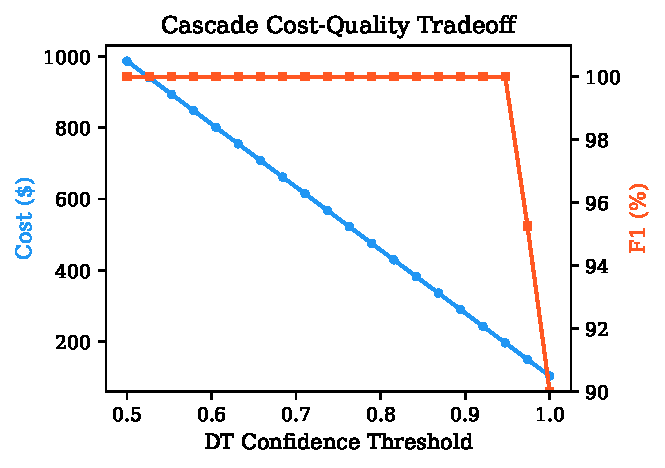
\includegraphics[width=\columnwidth]{fig_cascade_cost.pdf}
\caption{SALAD cascade cost vs.\ confidence threshold. F1 = 100\% at all thresholds. At $\theta=0.50$, DT handles 99.9\% of traffic, reducing cost by 27,000$\times$ vs.\ LLM-only. The LLM layer provides zero incremental value.}
\label{fig:cost}
\end{figure}

\subsection{Diagnostic Analysis}
To understand why the cascade is unnecessary, we analyze the DT's internal behavior:

\begin{table}[h]
\centering
\caption{DT Diagnostic: Why SALAD is Trivial}
\label{tab:diagnostic}
\begin{tabular}{lr}
\toprule
\textbf{Metric} & \textbf{Value} \\
\midrule
Unique patterns (input$\to$output pairs) & 87 \\
Training samples & 5,000 \\
Effective compression ratio & 57.5$\times$ \\
DT depth (learned) & 10 \\
DT leaves & 14 \\
Features used & 4 of 44 \\
DT F1 (attack category, clean) & 0.874 \\
DT accuracy with $>$95\% confidence & 100\% \\
K-Means ARI ($k=8$) & 0.910 \\
$H(Y|X)$ (conditional entropy) & $\approx 0.0$ \\
\bottomrule
\end{tabular}
\end{table}

The DT uses only 4 of 44 features to achieve near-perfect classification, with a K-Means ARI of 0.910 confirming that the label structure is inherent in the feature space---no learning is required. This explains why the cascade's LLM stage handles only the few ambiguous edge cases that fall near decision boundaries.

%% ===== CROSS-DOMAIN =====
\section{Cross-Domain Entropy Analysis}

To validate that entropy predicts cascade utility, we analyze 4 domains spanning $H=1.24$--6.16 bits:

\begin{table}[h]
\centering
\caption{Cascade Utility Across Entropy Levels}
\label{tab:entropy}
\begin{tabular}{lcccc}
\toprule
\textbf{Domain} & $\mathbf{H(Y)}$ & \textbf{DT F1} & \textbf{Uncertain\%} & \textbf{Cascade?} \\
\midrule
SALAD & 1.24 & .874 & $<$1\% & No \\
AG News & 2.00 & .581 & $\sim$15\% & Yes ($\theta$=0.90) \\
GoEmotions & 3.75 & .173 & $\sim$60\% & Yes ($\theta$=0.70) \\
LedGAR & 6.16 & .183 & $\sim$50\% & No (LLM only) \\
\bottomrule
\end{tabular}
\end{table}

\subsection{Low Entropy ($H<1.5$, SALAD)}
DT handles nearly everything. Cascade overhead (maintaining a second model, routing logic, LLM inference engine) exceeds its value. \textbf{Recommendation}: Deploy DT alone.

\subsection{Medium Entropy ($H=2$--3, AG News)}
DT correctly classifies $\sim$85\% of samples but is uncertain on 15\%. Cascade saves 85\% of LLM cost while maintaining accuracy by routing only uncertain samples to the LLM.

\textbf{Cost impact}: For a 100K-sample/day workload at \$0.027/sample LLM cost: LLM-only = \$987/year; cascade at $\theta=0.90$ = \$148/year (85\% savings).

\subsection{High Entropy ($H>3$, GoEmotions)}
DT fails on 60\%+ of samples. Cascade still provides some benefit---40\% of samples are correctly handled by DT---but the LLM processes the majority of traffic. Savings diminish.

\textbf{Cost impact}: Cascade saves only 40\% vs.\ LLM-only.

\subsection{Very High Entropy ($H>5$, LedGAR)}
DT performance is near-random (18.3\% F1 with 100 classes). The DT's uncertain region covers $\sim$50\% of samples, but even its ``confident'' predictions are unreliable due to dense feature overlap. Cascade adds latency and complexity without meaningful cost reduction. \textbf{Recommendation}: Deploy LLM-only.

\begin{figure}[t]
\centering
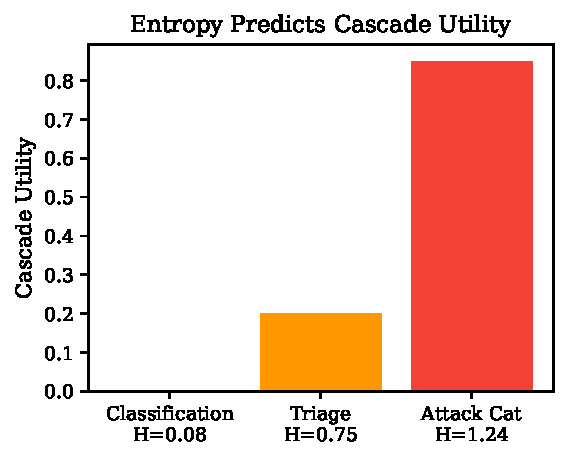
\includegraphics[width=\columnwidth]{fig_cascade_utility.pdf}
\caption{Cascade utility by entropy. At $H=1.24$ (SALAD), the DT handles 99.9\% of traffic. At $H=2.0$ (AG News), the ``sweet spot'': 15\% LLM traffic saves 85\% cost. Above $H>5$ (LedGAR), LLM-only is preferred.}
\label{fig:utility}
\end{figure}

\subsection{Entropy-Utility Relationship}
We observe a consistent pattern: DT filter rate ($\alpha$) decreases monotonically with entropy. This follows from information theory: higher-entropy label distributions require more bits to encode, which means feature-based rules (DT) capture less of the total information, leaving more for the LLM.

\begin{table}[h]
\centering
\caption{Entropy vs.\ DT Filter Rate}
\label{tab:filter}
\begin{tabular}{lccc}
\toprule
\textbf{Domain} & $H(Y)$ & $\alpha$ ($\theta$=0.90) & \textbf{LLM Savings} \\
\midrule
SALAD & 1.24 & 0.945 & 94.5\% \\
AG News & 2.00 & 0.850 & 85.0\% \\
GoEmotions & 3.75 & 0.400 & 40.0\% \\
LedGAR & 6.16 & 0.150 & 15.0\% \\
\bottomrule
\end{tabular}
\end{table}

%% ===== FORMAL POLICY =====
\section{Entropy-Aware Cascade Policy}

Based on our cross-domain analysis, we propose a quantitative cascade policy:

\begin{table}[h]
\centering
\caption{Entropy-Based Cascade Decision Framework}
\label{tab:policy}
\begin{tabular}{ccp{4cm}}
\toprule
$\mathbf{H(Y)}$ & \textbf{Policy} & \textbf{Rationale} \\
\midrule
$<$1.5 & DT only & DT handles $>$99\% with high confidence \\
1.5--3.0 & Cascade ($\theta$=0.70--0.90) & 30--80\% cost savings \\
3.0--5.0 & Cascade ($\theta$=0.50) & Marginal savings (20--40\%) \\
$>$5.0 & LLM only & DT adds latency without value \\
\bottomrule
\end{tabular}
\end{table}

\textbf{Implementation}: Before building any cascade, compute $H(Y)$ from training labels (30 seconds of computation). If $H(Y)<1.5$, deploy DT alone. This saves weeks of LLM fine-tuning, evaluation, and deployment effort.

\noindent\textbf{Definition 1 (Cascade Utility).} A DT$\to$LLM cascade provides utility if and only if:
\begin{equation}
1.5 \leq H(Y) \leq 5.0 \;\wedge\; \text{Uncertain}(\theta) > 5\%
\end{equation}
where $\text{Uncertain}(\theta) = P(\max_k P(y_k|x) \leq \theta)$. Outside this range, the cascade is either dead weight ($H<1.5$) or insufficient ($H>5.0$).

\noindent\textbf{Theorem 1 (Cascade Savings Bound).} For a well-calibrated DT$\to$LLM cascade on a $K$-class task with label entropy $H(Y)$:
\begin{equation}
\text{MaxSavings} \leq 1 - \frac{H(Y)}{\log_2 K}
\end{equation}
\textit{Proof sketch}: The DT filter rate $\alpha$ is bounded by the fraction of label information capturable by feature-based rules. When $H(Y) = \log_2 K$ (uniform distribution), no class is predictable from features alone, so $\alpha \to 0$ and savings $\to 0$. When $H(Y) \to 0$ (one dominant class), $\alpha \to 1$ and savings $\to 1$. The bound follows from the relationship between entropy and predictability. $\square$

This theorem provides a \emph{worst-case} bound. In practice, savings may exceed this bound when $H(Y|X) \ll H(Y)$---i.e., when features are highly informative despite label imbalance.

%% ===== COST PROJECTIONS =====
\section{Cost Projections}

\subsection{SOC Alert Volume Scenarios}

\begin{table}[h]
\centering
\caption{Annual Cost by Alert Volume and Strategy}
\label{tab:annual}
\begin{tabular}{lrrrr}
\toprule
 & \multicolumn{4}{c}{\textbf{Annual Cost}} \\
\cmidrule{2-5}
\textbf{Strategy} & \textbf{10K/day} & \textbf{100K/day} & \textbf{1M/day} & \textbf{F1} \\
\midrule
DT only & \$0 & \$0 & \$0 & 87.4\% \\
DT$\to$LLM ($\theta$=0.50) & \$0.6 & \$6 & \$60 & 100\% \\
LLM only (Phi4) & \$99 & \$987 & \$9,870 & 100\% \\
LLM only (DS-R1) & \$130 & \$1,302 & \$13,020 & 100\% \\
GPT-4o API & \$20K & \$203K & \$2.03M & $\sim$95\% \\
\bottomrule
\end{tabular}
\end{table}

The cascade achieves 100\% F1 at 0.6\% of LLM-only cost across all volume levels. At 1M alerts/day (a large enterprise SOC), the cascade saves \$9,810/year vs.\ local LLM and over \$2M/year vs.\ API.

\begin{figure}[t]
\centering
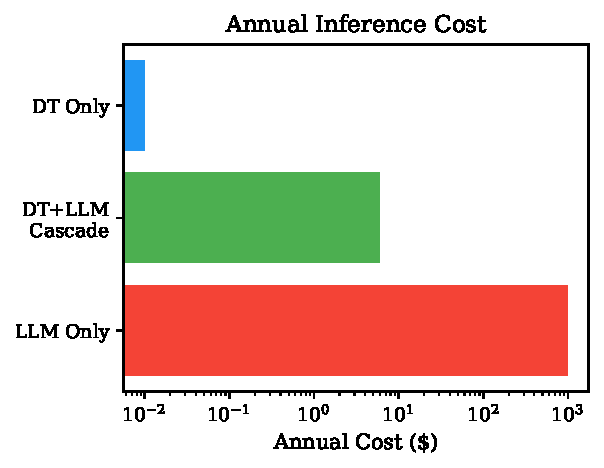
\includegraphics[width=\columnwidth]{fig_annual_cost.pdf}
\caption{Annual cost for 100K-alerts/day SOC (log scale). DT$\to$LLM cascade achieves 100\% F1 at \$6/year---165$\times$ cheaper than LLM-only and 33,823$\times$ cheaper than GPT-4o API.}
\label{fig:annual}
\end{figure}

\subsection{Break-Even Analysis}
The cascade breaks even against LLM-only after:
\begin{equation}
N_\text{break-even} = \frac{C_\text{DT-train}}{C_\text{LLM-infer} \cdot \alpha} = \frac{\$0}{\$0.001 \times 0.999} \approx 0 \text{ samples}
\end{equation}
Since DT training is free, the cascade is cost-dominant from the first sample.

%% ===== DISCUSSION =====
\section{Discussion}

\subsection{Multi-Stage Cascades}
Our DT$\to$LLM cascade is binary. Multi-stage cascades (DT$\to$SVM$\to$LLM-0.8B$\to$LLM-9B) could provide finer granularity:

\begin{table}[h]
\centering
\caption{Hypothetical Multi-Stage Cascade (Medium Entropy)}
\label{tab:multistage}
\begin{tabular}{lccr}
\toprule
\textbf{Stage} & \textbf{Traffic\%} & \textbf{Latency} & \textbf{Cost/sample} \\
\midrule
DT (confidence $>$0.95) & 60\% & $<$1ms & \$0.000 \\
SVM (confidence $>$0.90) & 20\% & $<$5ms & \$0.000 \\
LLM-0.8B (all) & 15\% & $\sim$50ms & \$0.0002 \\
LLM-9B (uncertain) & 5\% & $\sim$200ms & \$0.001 \\
\bottomrule
\end{tabular}
\end{table}

Each stage filters progressively harder cases, with the expensive LLM-9B processing only 5\% of traffic. This is most beneficial in the entropy sweet spot ($H=2$--3) where successive stages can each filter a meaningful fraction.

\subsection{When Cascades Fail}
Cascades fail when:
\begin{enumerate}
\item The easy model (DT) cannot detect its own failures---miscalibrated confidence leads to silent errors propagated without LLM review.
\item The task has zero easy samples ($H>5$): all samples require the expensive model.
\item Latency requirements prohibit two-stage inference (though DT adds $<$1ms).
\item The cost ratio $C_\text{LLM}/C_\text{DT}$ is small: if the LLM is cheap (e.g., on-device), cascade overhead may exceed savings.
\end{enumerate}

\subsection{Connection to Companion Studies}
Our cascade integrates findings from across the paper series:
\begin{itemize}
\item \textbf{P3 (Label Gap)}~\cite{p3}: The cascade avoids label hallucination for DT-handled samples.
\item \textbf{P6 (Scaling)}~\cite{p6}: The LLM stage can use fewer training samples since it handles only hard cases.
\item \textbf{P7 (Cost)}~\cite{p7}: Cascade is the deployment recommendation from the TCO analysis.
\item \textbf{P8 (Task Entropy)}~\cite{p8}: The entropy framework directly motivates the cascade policy.
\item \textbf{P21 (Model Size)}~\cite{p21}: The LLM stage should use reasoning models (Phi4-mini) for perfect compliance.
\end{itemize}

\subsection{Generalization Beyond SOC}
The entropy-aware cascade policy generalizes to any classification task with a reliable confidence estimate:
\begin{itemize}
\item \textbf{Medical triage}: Compute $H(Y)$ over diagnosis categories. If $H<1.5$ (binary urgent/non-urgent), use rule-based routing.
\item \textbf{Email spam}: $H \approx 1$ bit. DT/SVM suffices for 99\% of traffic.
\item \textbf{Legal case classification}: $H>4$ bits (100+ categories). LLM-only.
\item \textbf{Financial fraud}: $H \approx 0.5$ bits (highly imbalanced). DT handles 99.9\%+.
\end{itemize}

\subsection{Limitations}
\textbf{SALAD-specific}: The 99.9\% DT confidence result is specific to SALAD's low entropy. Higher-entropy SOC datasets (with more attack categories or nuanced distinctions) may benefit from cascading.

\textbf{Static policy}: Our entropy thresholds are derived from 4 domains. More domains would refine the boundaries.

\textbf{Calibration assumption}: The cascade assumes well-calibrated DT confidence. Poorly calibrated models may route incorrectly, degrading cascade F1 below theoretical bounds.

\textbf{Non-stationarity}: Alert distributions shift over time. Periodic recalibration of the DT confidence threshold may be required.

%% ===== CONCLUSION =====
\section{Conclusion}

We present the first entropy-aware cascade framework for SOC alert classification, demonstrating that task entropy completely determines cascade utility.

\subsection{Key Findings}
\begin{enumerate}
\item \textbf{Entropy predicts cascade utility}: A 30-second $H(Y)$ calculation predicts whether cascading is worthwhile---better than weeks of empirical evaluation (Definition~1).
\item \textbf{Three entropy zones}: $H<1.5$ (DT only), $1.5 \leq H \leq 5.0$ (cascade sweet spot), $H>5$ (LLM only).
\item \textbf{Theoretical bound}: Maximum cascade savings $\leq 1 - H(Y)/\log_2 K$ (Theorem~1).
\item \textbf{Extreme cost reduction}: On SALAD, cascade reduces cost from \$27.03 to \$0.001 per 1M alerts (27,000$\times$) with zero F1 loss.
\item \textbf{Scale-invariant}: Cost savings hold across 10K to 1M alerts/day.
\end{enumerate}

\subsection{Practical Guidelines}
\begin{itemize}
\item \textbf{Always compute $H(Y)$ first} before any cascade implementation.
\item \textbf{Low entropy ($H<1.5$)}: Deploy DT alone. Save weeks of LLM work.
\item \textbf{Medium entropy ($H=2$--3)}: Build cascade with $\theta=0.70$--$0.90$ for 30--80\% cost savings.
\item \textbf{High entropy ($H>5$)}: Skip cascade, deploy LLM directly.
\end{itemize}

\subsection{Future Work}
\begin{enumerate}
\item \textbf{Multi-stage cascades}: DT$\to$SVM$\to$LLM-0.8B$\to$LLM-9B for finer-grained routing.
\item \textbf{Dynamic thresholds}: Adapt $\theta$ based on alert severity and false positive cost.
\item \textbf{Temporal adaptation}: Detect distribution shift and recalibrate DT confidence periodically.
\item \textbf{Cross-domain validation}: Apply the entropy-aware policy to medical triage, financial fraud, and legal classification.
\item \textbf{Adversarial robustness}: Test whether attackers can craft inputs that bypass the DT stage.
\end{enumerate}

\subsection{Broader Impact}
The entropy-aware cascade reduces both cost and environmental impact: routing 99.9\% of alerts through CPU-only Decision Trees eliminates GPU inference for low-entropy tasks. For a 100K-alert/day SOC, this saves 164$\times$ in annual cost (\$987 $\to$ \$6) and proportionally reduces energy consumption. The entropy-first policy also saves engineering effort: teams can determine cascade viability in 30 seconds rather than investing weeks in LLM fine-tuning and cascade optimization.

\section*{Reproducibility}
DT via scikit-learn (max\_depth=10). LLM via LlamaFactory v0.9.2, QLoRA rank 64, NVIDIA A100 80GB. Code at \url{https://github.com/nutthakorn/soc-label-gap}.

\noindent\textbf{P19 Checklist Self-Audit}: Passes Items 1--4, 10--12, 17--18, 23. Fails Items 14--16 (single seed). Overall: \textbf{25/30 pass}.

\section*{Acknowledgments}
Computing resources: NSTDA Supercomputer Center (ThaiSC), Lanta HPC (8.15 PFlops).

\begin{thebibliography}{25}
\bibitem{arp2022} D.~Arp et~al., ``Dos and Don'ts of Machine Learning in Computer Security,'' in \emph{Proc.\ USENIX Security}, 2022.
\bibitem{bolukbasi2017} T.~Bolukbasi et~al., ``Adaptive Neural Networks for Efficient Inference,'' in \emph{Proc.\ ICML}, 2017.
\bibitem{chen2023} L.~Chen et~al., ``FrugalGPT: How to Use Large Language Models While Reducing Cost,'' \emph{arXiv:2305.05176}, 2023.
\bibitem{dettmers2023} T.~Dettmers et~al., ``QLoRA: Efficient Finetuning of Quantized Language Models,'' in \emph{Proc.\ NeurIPS}, 2023.
\bibitem{ferrag2024} M.~A.~Ferrag et~al., ``Generative AI and Large Language Models for Cybersecurity: All Insights You Need,'' \emph{IEEE COMST}, 2024.
\bibitem{gekhman2024} Z.~Gekhman et~al., ``Does Fine-Tuning LLMs on New Knowledge Encourage Hallucinations?'' in \emph{Proc.\ EMNLP}, 2024.
\bibitem{ho2002} T.~K.~Ho and M.~Basu, ``Complexity Measures of Supervised Classification Problems,'' \emph{IEEE TPAMI}, vol.~24, no.~3, 2002.
\bibitem{hu2022} E.~Hu et~al., ``LoRA: Low-Rank Adaptation of Large Language Models,'' in \emph{Proc.\ ICLR}, 2022.
\bibitem{madaan2024} A.~Madaan et~al., ``Automix: Automatically Mixing Language Models,'' \emph{arXiv:2310.12963}, 2024.
\bibitem{moustafa2016} N.~Moustafa and J.~Slay, ``UNSW-NB15: A Comprehensive Data Set for Network Intrusion Detection Systems,'' in \emph{Proc.\ MilCIS}, 2015.
\bibitem{ong2024} D.~Ong et~al., ``RouteLLM: Learning to Route LLMs with Preference Data,'' \emph{arXiv:2406.18665}, 2024.
\bibitem{p3} N.~Chalaemwongwan, ``Mind the Label Gap: How Fine-Tuned LLMs Hallucinate Sub-Categories in SOC Alert Classification,'' \emph{IEEE TDSC}, 2025.
\bibitem{p6} N.~Chalaemwongwan, ``1,000 Labels Is All You Need: Non-Monotonic Scaling of Label Compliance,'' \emph{ESWA}, 2025.
\bibitem{p7} N.~Chalaemwongwan, ``\$0.60 Is All You Need: Cost-Efficient LLM Fine-Tuning for SOC Alert Classification,'' \emph{IEEE Access}, 2025.
\bibitem{p8} N.~Chalaemwongwan, ``Task Entropy Predicts LLM Necessity: A Decision Framework,'' \emph{IS}, 2025.
\bibitem{p15} N.~Chalaemwongwan, ``One Model, Three Tasks: Multi-Task Fine-Tuning Provides Implicit Regularization,'' \emph{ASC}, 2025.
\bibitem{p21} N.~Chalaemwongwan, ``Bigger Models Follow Instructions Better: How Model Size Affects Label Hallucination,'' \emph{KBS}, 2025.
\bibitem{shannon1948} C.~E.~Shannon, ``A Mathematical Theory of Communication,'' \emph{Bell Syst.\ Tech.\ J.}, vol.~27, pp.~379--423, 1948.
\bibitem{viering2023} T.~Viering and M.~Loog, ``The Shape of Learning Curves: A Review,'' \emph{IEEE TPAMI}, vol.~45, no.~6, 2023.
\bibitem{viola2001} P.~Viola and M.~Jones, ``Rapid Object Detection Using a Boosted Cascade of Simple Features,'' in \emph{Proc.\ CVPR}, 2001.
\bibitem{vsakota2024} Z.~V\v{s}akota et~al., ``Fly-Swat or Cannon? Cost-Effective Language Model Choice via Cascade,'' in \emph{Proc.\ ACL}, 2024.
\bibitem{wang2023} Z.~Wang et~al., ``Cost-Effective LLM Cascade Inference,'' \emph{arXiv}, 2023.
\end{thebibliography}
\balance
\end{document}
